\documentclass[12pt,a4paper]{article}

% Paquetes básicos
\usepackage[utf8]{inputenc}
\usepackage[spanish,es-tabla]{babel}

% Formato APA 7 (márgenes y tipografía)
\usepackage{geometry}
\geometry{a4paper, left=2.54cm, right=2.54cm, top=2.54cm, bottom=2.54cm}
\usepackage{times} 
\usepackage{setspace}
\setstretch{1.5} % Espacio y medio para legibilidad y volumen

% Paquetes gráficos y de tablas
\usepackage{graphicx}
\usepackage{float}
\usepackage{booktabs}
\usepackage{tabularx}
\usepackage{caption}
\captionsetup[table]{labelsep=newline, textfont=it, labelfont=bf, justification=raggedright, singlelinecheck=false}
\captionsetup[figure]{labelsep=newline, textfont=it, labelfont=bf, justification=raggedright, singlelinecheck=false}
\usepackage{subcaption}
\usepackage{pdflscape} % Para tablas apaisadas si es necesario

% Matemáticas
\usepackage{amsmath}
\usepackage{amsfonts}
\usepackage{amssymb}

% Paquetes para código fuente y algoritmos
\usepackage{listings}
\usepackage{xcolor}
\usepackage{algorithm}
\usepackage{algpseudocode}

\definecolor{codegreen}{rgb}{0,0.6,0}
\definecolor{codegray}{rgb}{0.5,0.5,0.5}
\definecolor{codepurple}{rgb}{0.58,0,0.82}
\definecolor{backcolour}{rgb}{0.95,0.95,0.92}

\lstdefinestyle{mystyle}{
    backgroundcolor=\color{backcolour},   
    commentstyle=\color{codegreen},
    keywordstyle=\color{blue},
    numberstyle=\tiny\color{codegray},
    stringstyle=\color{codepurple},
    basicstyle=\ttfamily\footnotesize,
    breakatwhitespace=false,         
    breaklines=true,                 
    captionpos=b,                    
    keepspaces=true,                 
    numbers=left,                    
    numbersep=5pt,                  
    showspaces=false,                
    showstringspaces=false,
    showtabs=false,                  
    tabsize=2
}
\lstset{style=mystyle}

% Enlaces
\usepackage[hidelinks]{hyperref}

% Diagramas de Flujo
\usepackage{tikz}
\usetikzlibrary{shapes.geometric, arrows, positioning, babel}

\begin{document}

% ==========================================
% PORTADA
% ==========================================
\begin{titlepage}
    \centering
    \vspace*{1cm}
    
    {\fontsize{14}{16}\selectfont \textbf{Universidad Nacional del Altiplano}\par}
    \vspace{0.5cm}
    {\fontsize{12}{14}\selectfont Facultad de Ingeniería Mecánica Eléctrica, Electrónica y Sistemas\par}
    \vspace{0.3cm}
    {\fontsize{12}{14}\selectfont Escuela Profesional de Ingeniería de Sistemas\par}
    
    \vspace{1.5cm}
    
    
\includegraphics[width=4.5cm]{figuras/logo.png} % 📸 [IMAGEN 1]: Logo de la UNA
    
    \vspace{1.5cm}
    
    {\fontsize{18}{22}\selectfont \textbf{Simulador del Núcleo del Sistema Operativo}\par}
    
    \vspace{2cm}
    
    \begin{tabular}{rl}
        \textbf{Autor:} & Abad Poma Maquera \\
        [0.3cm]
        \textbf{Código de Matrícula:} & 241177 \\
        [0.3cm]
        \textbf{Curso:} & SIS215 – Sistemas Operativos \\
        [0.3cm]
        \textbf{Docente:} & Ruelas Acero Donia Alizandra \\
    \end{tabular}
    
    \vfill
    
    {\fontsize{12}{14}\selectfont Puno, Perú\par}
    \vspace{0.3cm}
    {\fontsize{12}{14}\selectfont 2026\par}
\end{titlepage}

\newpage

% ==========================================
% ÍNDICE
% ==========================================
\tableofcontents
\newpage

% ==========================================
% 1. INTRODUCCIÓN Y OBJETIVOS
% ==========================================
\section{Introducción y Objetivos}

\subsection{Introducción}

El estudio de los Sistemas Operativos (SO) es esencial para comprender el diseño de software y la administración del hardware. Un SO funciona como un administrador central encargado de repartir recursos limitados frente a múltiples tareas simultáneas (Silberschatz, Galvin, \& Gagne, 2018). Dentro de esta arquitectura, la optimización de la Unidad Central de Procesamiento (CPU), la Memoria Principal y el Almacenamiento Secundario (Disco) determina el rendimiento general de los equipos de cómputo (Tanenbaum \& Bos, 2015). Dado el alto nivel de abstracción de estos mecanismos, su evaluación puramente teórica presenta dificultades para observar el comportamiento dinámico en tiempo real, requiriendo plataformas que permitan la experimentación práctica (Stallings, 2018).

Bajo este contexto, se expone SimuKernel, un entorno de simulación web interactivo que agrupa los tres componentes fundamentales del núcleo del SO: planificación de CPU, asignación de memoria y gestión de disco. El sistema visualiza la ejecución de diversos algoritmos clásicos basándose en un avance por ciclos de reloj (ticks). Al dividir la plataforma en módulos especializados, se viabiliza la recolección empírica de métricas de rendimiento y se permite una observación directa de las estructuras de datos que rigen el procesamiento interno del ordenador.

\subsection{Objetivo General}
Desarrollar un simulador web unificado que integre los algoritmos de planificación de CPU, asignación de Memoria Principal y gestión de Disco Secundario, proporcionando un entorno interactivo para la evaluación empírica de su rendimiento en tiempo real.

\subsection{Objetivos Específicos}
\begin{itemize}
    \item Programar el planificador de CPU para los algoritmos FCFS, SJF, SRT y Round Robin, calculando métricas de tiempos de espera y retorno.
    \item Diseñar un módulo visual para la asignación de Memoria Principal aplicando las estrategias First Fit, Best Fit, Worst Fit y Buddy System.
    \item Implementar siete métodos de asignación de Disco (Contigua, Enlazada, Indexada, FAT, Multinivel, Extensiones y Mapa de Bits) evaluando la fragmentación y el costo estructural.
    \item Extraer y tabular los indicadores de rendimiento de cada componente, tales como fragmentación, uso de capacidad y operaciones de E/S.
    \item Estructurar una interfaz gráfica interactiva y libre de dependencias externas complejas, asegurando su compatibilidad nativa en navegadores web.
    \item Generar representaciones visuales instantáneas de las estructuras subyacentes a través de diagramas de Gantt, mapas de bits y cuadrículas espaciales.
\end{itemize}

% ==========================================
% 2. MARCO TEÓRICO
% ==========================================
\section{Marco Teórico}

El núcleo de un sistema operativo opera como el administrador absoluto del hardware subyacente. Para comprender plenamente las decisiones de diseño adoptadas en la construcción del simulador, resulta imperativo explorar los fundamentos matemáticos y conceptuales que rigen la administración de los recursos críticos. En los siguientes apartados se desglosa la teoría algorítmica detrás de la gestión del procesador, la memoria principal y el disco magnético, contextualizando cada método con su aplicación real en la computación.

\subsection{Planificación de CPU}
El procesador es el recurso de cálculo más valioso dentro de la arquitectura de computadoras. La planificación del procesador constituye la base de la multiprogramación, cuyo propósito es maximizar el uso de la CPU y mejorar la capacidad de respuesta de los sistemas interactivos (Silberschatz et al., 2018). El desafío principal radica en arbitrar de manera justa y eficiente el acceso a la unidad de procesamiento frente a múltiples tareas que compiten simultáneamente. Todo proceso pasa por un ciclo vital conformado por los estados de Nuevo, Listo, En Ejecución, En Espera y Terminado. El despachador transfiere el control de la CPU al proceso seleccionado por el planificador de corto plazo, siendo imperativo minimizar el tiempo perdido en el cambio de contexto (Stallings, 2018).

\subsubsection{Algoritmos}

\paragraph{First-Come, First-Served (FCFS)}
Se asigna la CPU al primer proceso que la solicita, administrando la cola como una estructura FIFO estricta y sin expulsión. Su debilidad es el efecto convoy, donde tareas cortas quedan atrapadas tras un proceso intensivo (Arpaci-Dusseau \& Arpaci-Dusseau, 2018). Por ejemplo, si se consideran tres procesos con ráfagas de 24, 3 y 3 milisegundos que llegan en el orden P1, P2, P3, el algoritmo ejecutará P1 por 24 ms, retrasando significativamente a P2 y P3 y elevando el tiempo de espera (Silberschatz et al., 2018).

\paragraph{Shortest Job First (SJF)}
Se asocia a cada proceso la duración de su siguiente ráfaga de CPU y se selecciona al de menor duración en modo no expulsivo (Silberschatz et al., 2018). Por ejemplo, si los procesos P1, P2 y P3 tienen ráfagas de 8, 4 y 2 milisegundos y se encuentran listos, el sistema ejecutará P3, seguido de P2 y finalmente P1, reduciendo el tiempo de espera frente a FCFS (Stallings, 2018).

\paragraph{Shortest Remaining Time (SRT)}
Constituye la variante expulsiva de SJF. Ante la llegada de un nuevo proceso, se evalúa su ráfaga contra el tiempo restante del proceso actual. Si la nueva es menor, ocurre un cambio de contexto (Stallings, 2018). A modo de ejemplo, si un proceso P1 de 10 ms lleva 2 ms en CPU y llega un proceso P2 de 4 ms, el sistema interrumpe a P1 (8 ms restantes) para ejecutar inmediatamente a P2, minimizando el tiempo de respuesta (Love, 2010).

\paragraph{Round Robin (RR)}
La cola de listos se administra de forma circular, asignando una fracción de tiempo fija denominada quantum (Corbató, 1962). Si la ráfaga supera el quantum, el proceso es interrumpido coercitivamente. Por ejemplo, con un quantum de 4 ms, si un proceso requiere 10 ms, ejecutará 4 ms, será enviado al final de la cola, y esperará su próximo turno para ejecutar los siguientes milisegundos (Tanenbaum \& Bos, 2015).

\subsection{Gestión de Memoria Principal}
La memoria administra el espacio dual entre direcciones lógicas y físicas, utilizando políticas del SO para su traducción y particionamiento (Denning, 1970).

\subsubsection{Algoritmos}

\paragraph{Algoritmos de Asignación Contigua Dinámica}
Se asignan bloques ajustados exactamente a la necesidad del proceso:
\begin{itemize}
    \item \textbf{First Fit:} Asigna el primer hueco suficientemente grande. Por ejemplo, al solicitar 15 KB en una memoria con huecos libres de 10 KB, 20 KB y 15 KB en orden, se asignará en el bloque de 20 KB por ser el primero válido, dejando 5 KB libres (Silberschatz et al., 2018).
    \item \textbf{Best Fit:} Escudriña toda la memoria y selecciona el hueco más pequeño que satisfaga la petición. Utilizando el ejemplo anterior de 15 KB con huecos de 10, 20 y 15 KB, se asignará exactamente en el bloque de 15 KB, sin dejar residuo inmediato (Tanenbaum \& Bos, 2015).
    \item \textbf{Worst Fit:} Elige el hueco de mayor tamaño. En el mismo escenario, si el hueco más grande es de 50 KB, se asignarán los 15 KB allí, generando un sobrante de 35 KB destinado a futuros procesos (Stallings, 2018).
\end{itemize}

\paragraph{Sistema Colega (Buddy System)}
Se resuelve la asignación dividiendo la memoria iterativamente a la mitad, operando en bloques con tamaños de potencias de 2 (Knuth, 1997). Por ejemplo, si se solicitan 20 KB, el sistema divide un bloque inicial de 64 KB en dos de 32 KB y asigna uno de ellos, causando 12 KB de fragmentación interna. Al liberarse, si el bloque colega de 32 KB está libre, se fusionan nuevamente en 64 KB (Silberschatz et al., 2018).

\subsection{Gestión de Almacenamiento Secundario (Disco)}
El disco se gestiona mediante algoritmos enfocados en contigüidad y metadatos (Tanenbaum \& Bos, 2015).

\subsubsection{Algoritmos}

\paragraph{Asignación Contigua}
El directorio almacena el bloque inicial y la longitud. Por ejemplo, un archivo de 5 bloques que inicia en el bloque 10 ocupará estrictamente del 10 al 14. Ofrece rendimiento óptimo, pero genera fragmentación externa masiva si el archivo requiere expansión y no hay espacio adyacente (Stallings, 2018).

\paragraph{Asignación Enlazada}
Se conforma una lista enlazada de bloques físicos. Por ejemplo, un archivo de 3 bloques puede ocupar los bloques 8, 1 y 15, donde el bloque 8 contiene un puntero al 1, y el 1 al 15. Se evita la fragmentación externa, pero se sacrifica el acceso aleatorio y se incurre en gasto estructural (Silberschatz et al., 2018).

\paragraph{Asignación Indexada}
Se agrupan los punteros en un bloque de índice. Por ejemplo, para un archivo disperso en los bloques 4, 19 y 2, el bloque índice número 10 contendrá las direcciones 4, 19 y 2. Esto permite acceso aleatorio directo al penalizar el almacenamiento con un bloque entero para metadatos (Tanenbaum \& Bos, 2015).

\paragraph{FAT (File Allocation Table)}
Los punteros se trasladan a una tabla centralizada en memoria. Por ejemplo, si un archivo inicia en el bloque 5 y sigue en el 12, la entrada 5 de la tabla FAT contendrá el valor 12. Esto acelera la navegación y disminuye las lecturas magnéticas sucesivas (Arpaci-Dusseau \& Arpaci-Dusseau, 2018).

\paragraph{Indexada Multinivel}
Un bloque índice principal apunta a bloques secundarios. Por ejemplo, un archivo masivo llena un bloque índice primario con 256 punteros que dirigen a bloques índice secundarios; estos, a su vez, apuntan a los datos reales, permitiendo escalar a tamaños teóricamente inmensos sin requerir contigüidad (McKusick et al., 1984).

\paragraph{Extensiones (Extents)}
Se registra una tupla de inicio y longitud. Por ejemplo, un archivo de 1000 bloques continuos que inicia en el sector 50 se representa únicamente como (50, 1000), comprimiendo el almacenamiento de metadatos radicalmente en comparación con listar 1000 punteros (Mathur et al., 2007).

\paragraph{Mapa de Bits (Bitmap)}
Se representa cada sector físico como un bit. Por ejemplo, una secuencia de bits 110001 indica que los bloques 0, 1 y 5 están ocupados, mientras que 2, 3 y 4 están libres. Se utiliza para localizar espacios vacíos contiguos a gran velocidad mediante instrucciones de procesador (Silberschatz et al., 2018).

% ==========================================
% 3. METODOLOGÍA
% ==========================================
\section{Metodología}

La construcción y evaluación del simulador se rigió por un enfoque de desarrollo de software incremental y una posterior experimentación cuantitativa. Para garantizar la fiabilidad técnica del sistema, el trabajo empírico se estructuró en tres fases metodológicas orientadas netamente a la ingeniería de software y al análisis de algoritmos.

\subsection{Desarrollo Iterativo y Modular}
La construcción del núcleo adoptó un ciclo de vida iterativo, permitiendo la implementación aislada de los módulos de procesamiento, almacenamiento primario y almacenamiento secundario. Esta estricta separación arquitectónica asegura que la lógica matemática de cada componente opere de manera independiente. De esta forma, se facilita la depuración a bajo nivel y se garantiza que el estado de la memoria RAM no contamine el flujo del planificador de CPU durante la simulación.

\subsection{Implementación de Estructuras Abstractas}
En lugar de depender de librerías externas que abstraen la complejidad computacional, el motor lógico se desarrolló desde cero empleando tipos de datos fundamentales. Se programaron colas de prioridad dinámicas para simular el despachador de procesos, árboles binarios particionados para el modelo Buddy System de memoria, y matrices de asignación bidimensionales para emular la superficie de los clústeres magnéticos del disco. Este enfoque algorítmico garantiza que el rendimiento medido provenga estrictamente de la eficiencia del código y no de optimizaciones ocultas provistas por lenguajes de alto nivel.

\subsection{Evaluación Empírica por Lotes}
Para validar la funcionalidad y estabilidad de los algoritmos implementados, se diseñó un modelo de estrés basado en la inyección de conjuntos de datos estandarizados (procesamiento por lotes). Cada lote de prueba contiene parámetros estáticos de tiempos de llegada y requerimientos de memoria. Al someter todos los algoritmos exactamente a las mismas condiciones iniciales, se logró extraer comparativas puramente deterministas, permitiendo registrar de forma fidedigna el comportamiento del sistema frente a la fragmentación severa y escenarios de inanición.

% ==========================================
% 4. MÉTRICAS DE EVALUACIÓN
% ==========================================
\section{Métricas de Evaluación}

\subsection{Métricas de CPU}
Sea un conjunto de procesos $P = \{P_1, P_2, \dots, P_n\}$. Para cada proceso $P_i$ se definen las variables primitivas: $t_{llegada}(P_i)$, $t_{rafaga}(P_i)$, $t_{finalizacion}(P_i)$ y $t_{inicio}(P_i)$ (Silberschatz et al., 2018). Las métricas calculadas por el simulador son:

\begin{itemize}
    \item \textbf{Total Procesos:} Conteo absoluto de entidades admitidas al planificador.
    \item \textbf{Uso de CPU (\%):} Fracción del tiempo en que el procesador ejecutó instrucciones de usuario. Un valor cercano al 100\% indica una alta eficiencia en la multiprogramación y una reducción en la inactividad del hardware (Stallings, 2018):
    \begin{equation}
        U = \left( \frac{\sum_{i=1}^{n} t_{rafaga}(P_i)}{\text{Tiempo Total de Simulación}} \right) \times 100\%
    \end{equation}
    \item \textbf{Tiempo de Espera Promedio ($\overline{T_{esp}}$):} Tiempo que cada proceso permaneció inactivo en la cola de Listos. Se utiliza para medir la penalización que el despachador impone sobre los procesos (Tanenbaum \& Bos, 2015):
    \begin{equation}
        T_{esp}(P_i) = T_{ret}(P_i) - t_{rafaga}(P_i)
    \end{equation}
    \item \textbf{Tiempo de Retorno Promedio ($\overline{T_{ret}}$):} Intervalo total desde la llegada hasta la finalización. Permite evaluar el lapso global para la culminación de un ciclo de trabajo (Silberschatz et al., 2018):
    \begin{equation}
        T_{ret}(P_i) = t_{finalizacion}(P_i) - t_{llegada}(P_i)
    \end{equation}
    \item \textbf{Tiempo de Respuesta ($T_{res}$):} Lapso desde la llegada hasta la primera ejecución en CPU. Es crítico en sistemas interactivos donde la respuesta temprana previene bloqueos aparentes (Arpaci-Dusseau \& Arpaci-Dusseau, 2018):
    \begin{equation}
        T_{res}(P_i) = t_{inicio}(P_i) - t_{llegada}(P_i)
    \end{equation}
    \item \textbf{Throughput ($X$):} Tasa de procesos completados por unidad de tiempo. Representa el rendimiento volumétrico del procesador (Stallings, 2018):
    \begin{equation}
        X = \frac{n}{\max(t_{finalizacion})} \text{ procesos/unidad de tiempo}
    \end{equation}
\end{itemize}

\subsection{Métricas de Memoria}
Basadas estrictamente en la función \texttt{calcularMetricasMemoria} del simulador, sean $S(P_i)$ el tamaño solicitado por el proceso $i$, $A(P_i)$ el tamaño del bloque asignado, y $Mem_{total}$ la capacidad total de la RAM (Silberschatz et al., 2018):

\begin{itemize}
    \item \textbf{Uso de RAM (\texttt{porcentajeUso}):} Porcentaje de la memoria ocupada por datos útiles de procesos. Cuantifica el éxito de las políticas de retención y despacho (Tanenbaum \& Bos, 2015):
    \begin{equation}
        U_m = \left( \frac{\texttt{kbUsados}}{Mem_{total} - Mem_{SO}} \right) \times 100\%
    \end{equation}
    \item \textbf{Memoria Libre:} Cantidad total de KB disponibles para nuevas asignaciones.
    \item \textbf{Fragmentación Interna (\texttt{fragInterna}):} Desperdicio acumulado dentro de los bloques asignados cuando $A(P_i) > S(P_i)$. Se evalúa para exponer ineficiencias en particionamientos rígidos como el Buddy System (Knuth, 1997):
    \begin{equation}
        F_{int} = \sum_{i=1}^{n} \left( A(P_i) - S(P_i) \right)
    \end{equation}
    \item \textbf{Fragmentación Externa (\texttt{fragExterna}):} Suma total del espacio libre disperso en múltiples huecos no contiguos. Refleja la imposibilidad de utilizar memoria total disponible, requiriendo algoritmos de compactación (Stallings, 2018):
    \begin{equation}
        F_{ext} = \sum_{j=1}^{m} \text{tamaño}(h_j) \quad \text{donde } h_j \text{ son los huecos libres}
    \end{equation}
    \item \textbf{Procesos Asignados (\texttt{procesosAsignados}):} Relación entre procesos exitosamente cargados y el total de solicitudes.
\end{itemize}

\subsection{Métricas de Disco}
Basadas estrictamente en la función \texttt{calcularMetricasDisco} del simulador. El rendimiento del almacenamiento secundario se evalúa con las siguientes métricas, diseñadas para reflejar restricciones físicas y estructurales (Stallings, 2018):

\begin{itemize}
    \item \textbf{Bloques Ocupados (\texttt{bloquesOcupados}):} Total de bloques del disco utilizados por datos y metadatos, midiendo la densidad de empaquetado (Tanenbaum \& Bos, 2015).
    \item \textbf{Bloques Libres (\texttt{bloquesLibres}):} Cantidad de bloques vacíos y disponibles.
    \item \textbf{\% Uso Disco:} Proporción de bloques ocupados respecto del total.
    \item \textbf{Archivos Activos (\texttt{archivosSet}):} Conteo de archivos distintos actualmente almacenados.
    \item \textbf{Fragmentación Externa:} Conteo de huecos libres discontinuos. Un valor alto alerta sobre la degradación futura en la asignación contigua (Silberschatz et al., 2018).
    \item \textbf{Op. E/S (R:W):} Lecturas y escrituras acumuladas a nivel de bloque, modelando el costo electromecánico del hardware físico (Arpaci-Dusseau \& Arpaci-Dusseau, 2018).
\end{itemize}

Adicionalmente, para evaluar el impacto estructural de los metadatos se emplea el \textbf{Overhead} ($O_d$) (McKusick et al., 1984):
\begin{equation}
    O_d = \left( \frac{B_{meta}}{B_{meta} + B_{datos}} \right) \times 100\%
\end{equation}
donde $B_{meta}$ son los bloques de metadatos (punteros, tablas FAT, bloques índice) y $B_{datos}$ los bloques de contenido útil.

El Tiempo de Acceso Total a un bloque físico en un HDD se modela integrando los tiempos de búsqueda y mecánicos (Silberschatz et al., 2018):
\begin{equation}
    T_a = T_s + T_r + T_t
\end{equation}
donde $T_s$ es el \textit{Seek Time}, $T_r$ la \textit{Latencia Rotacional} y $T_t$ el \textit{Tiempo de Transferencia}.

% ==========================================
% 5. ARQUITECTURA Y DISEÑO DEL SIMULADOR
% ==========================================
\section{Arquitectura y Diseño del Simulador}

\subsection{Tecnologías y Estructura del Código}
El simulador se desarrolló íntegramente en Vanilla JS para maximizar el rendimiento de ejecución sin depender de bibliotecas de terceros que puedan introducir sobrecarga o retrasos asíncronos impredecibles. Se empleó HTML5 Canvas para el renderizado eficiente de las estructuras espaciales, posibilitando la manipulación geométrica a bajo nivel para representar la memoria y los sectores del disco. Para la estructuración visual, se implementaron Variables CSS, permitiendo una adaptación dinámica del entorno gráfico. 

Se implementó un sistema de Modo Oscuro/Claro basado en la mutación de variables CSS directamente en la raíz del documento (\texttt{:root}). Al accionar el interruptor de tema, el motor intercepta el evento y reasigna los códigos de color globales sin requerir la recarga del navegador ni el repintado del Canvas desde cero. Este modelo garantiza una transición fluida y mantiene intacto el estado interno de la simulación.

\subsection{Flujo de Ejecución del Sistema}

\begin{figure}[H]
    \centering
    \begin{tikzpicture}[node distance=2cm, auto, thick, scale=0.8, every node/.style={transform shape}]
        \tikzstyle{startstop} = [rectangle, rounded corners, minimum width=3cm, minimum height=1cm, text centered, draw=black, fill=gray!20]
        \tikzstyle{process} = [rectangle, minimum width=3cm, minimum height=1cm, text centered, draw=black, fill=blue!10]
        \tikzstyle{decision} = [diamond, aspect=2, minimum width=3cm, minimum height=1cm, text centered, draw=black, fill=orange!20]
        \tikzstyle{arrow} = [thick,->,>=stealth]

        \node (start) [startstop] {Inicio};
        \node (sel) [decision, below of=start, yshift=-1cm] {Selección de Módulo};
        
        \node (inyeccion) [process, below left=1cm and 2cm of sel] {Ingreso de Procesos};
        \node (cpu) [process, below of=inyeccion] {Planificador de CPU};
        \node (memoria) [process, below of=cpu] {Asignación Sincronizada de Memoria};
        
        \node (archivos) [process, below right=1cm and 2cm of sel] {Ingreso de Archivos};
        \node (disco) [process, below of=archivos] {Asignación y Mapeo en Disco};
        
        \node (metricas) [process, below of=sel, yshift=-7cm] {Extracción y Renderizado de Métricas};
        \node (stop) [startstop, below of=metricas] {Fin};

        \draw [arrow] (start) -- (sel);
        \draw [arrow] (sel) -| node[anchor=south, xshift=1.5cm] {CPU + MEM} (inyeccion);
        \draw [arrow] (sel) -| node[anchor=south, xshift=-1.5cm] {DISCO} (archivos);
        
        \draw [arrow] (inyeccion) -- (cpu);
        \draw [arrow] (cpu) -- (memoria);
        \draw [arrow] (memoria) |- (metricas);
        
        \draw [arrow] (archivos) -- (disco);
        \draw [arrow] (disco) |- (metricas);
        
        \draw [arrow] (metricas) -- (stop);
    \end{tikzpicture}
    \caption{Diagrama de Flujo del Simulador (Enfoque Modular Bifurcado)}
    \par\vspace{0.2cm}\raggedright \textit{Nota.} Esta figura ilustra la arquitectura de procesamiento bifurcado del simulador, diferenciando la ejecución conjunta de CPU y Memoria frente al tratamiento del disco, culminando en un motor unificado de extracción de métricas.
\end{figure}

La Figura 1 esquematiza el diseño algorítmico del núcleo, el cual sigue un trazado bifurcado. Desde la selección inicial, el flujo de procesamiento diverge hacia la simulación conjunta de CPU y Memoria (donde las tareas atraviesan el despachador y el particionamiento de RAM de forma sincronizada) o hacia el módulo dedicado de Almacenamiento Secundario (para la evaluación de metadatos y fragmentación en disco). Ambos caminos estructurales convergen de manera determinista en un único motor de extracción y renderizado de métricas.

\subsection{Interfaz Gráfica}
El diseño visual se priorizó para ofrecer una experiencia analítica directa, separando los paneles de control de los elementos de renderizado.

\begin{figure}[H] 
    \centering 
    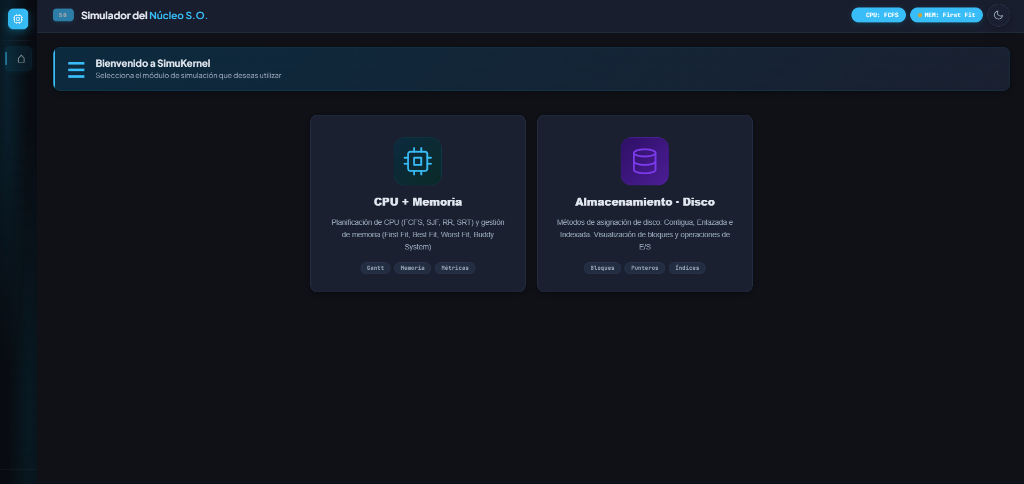
\includegraphics[width=0.9\linewidth]{figuras/IMAGEN_2.png} 
    \caption{Pantalla de inicio del simulador operando en Modo Oscuro.} 
    \par\vspace{0.2cm}\raggedright \textit{Nota.} Esta figura muestra la interfaz gráfica principal de la herramienta, resaltando la organización en módulos independientes y la aplicación de variables CSS para el contraste visual adecuado en modo oscuro.
\end{figure}

La Figura 2 detalla el menú principal de acceso al sistema, estructurado en dos grandes módulos independientes. La arquitectura de navegación bifurca la ejecución conjunta de CPU y Memoria frente a la evaluación dedicada del Almacenamiento Secundario. El diseño implementa variables CSS dinámicas para consolidar el contraste visual del entorno oscuro, reduciendo la fatiga visual durante sesiones prolongadas y acelerando el ingreso a los entornos de renderizado mediante indicadores gráficos de acceso rápido.

Una vez dentro de los módulos, el panel lateral despliega los controles paramétricos (ver Figura 3). Estos paneles permiten inyectar dinámicamente los tiempos de ráfaga, llegada, tamaños de solicitud y seleccionar las políticas algorítmicas sin recargar la página.

\begin{figure}[H]
    \centering
    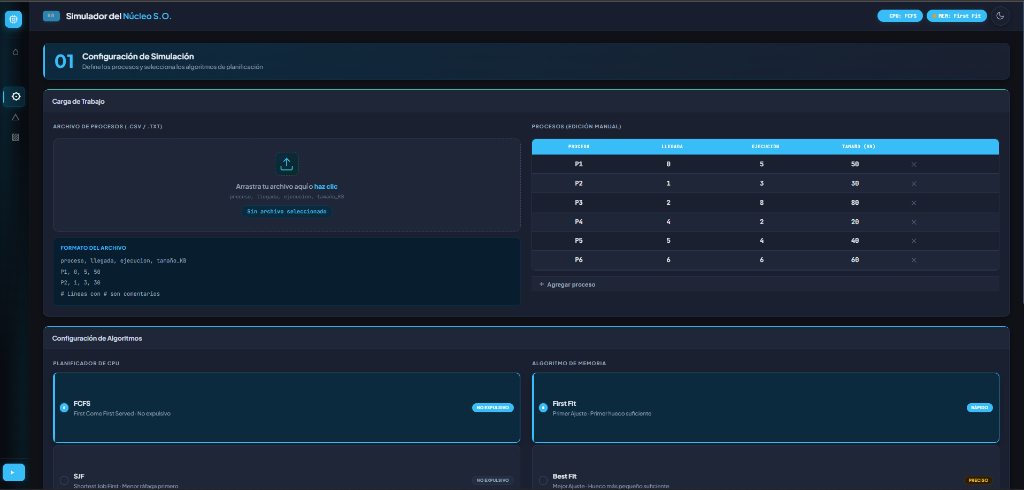
\includegraphics[width=1\linewidth]{figuras/IMAGEN_PARAM_CPU.png}
    \vspace{0.5cm}

    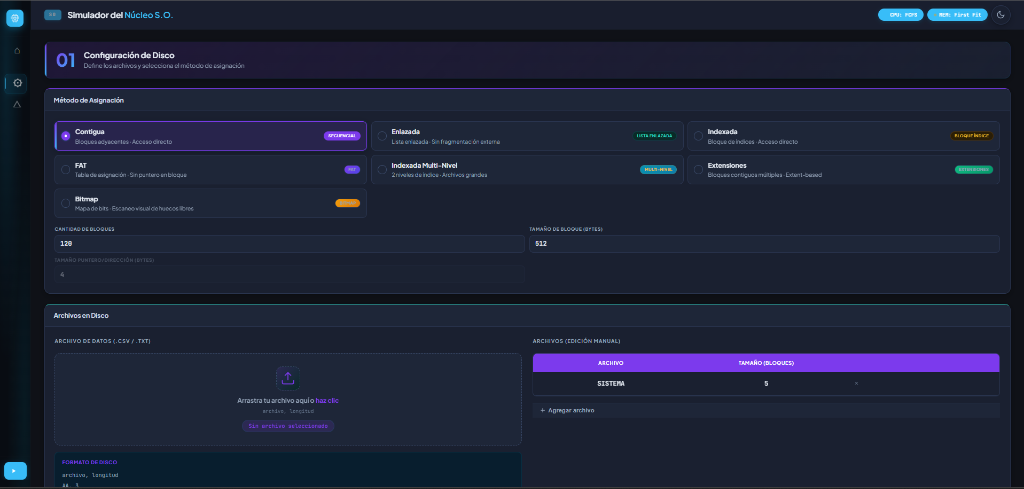
\includegraphics[width=1\linewidth]{figuras/IMAGEN_PARAM_DISCO.png}
    \caption{Paneles de configuración paramétrica para CPU/Memoria (arriba) y Disco (abajo)}
    \par\vspace{0.2cm}\raggedright \textit{Nota.} La figura detalla los paneles de control utilizados para la inyección de cargas de trabajo. Se observa la parametrización dinámica de ráfagas, tiempos de llegada y tamaños de archivo para su evaluación en los distintos algoritmos.
\end{figure}

\subsection{Implementación Algorítmica}
Se extraen a continuación los segmentos algorítmicos fundamentales que rigen el motor del simulador. 

\subsubsection{Algoritmos de CPU}

\begin{lstlisting}[language=Java, caption={FCFS (First-Come, First-Served)}]
    const tiempoInicio = tiempoActual;
    const tiempoFin    = tiempoActual + proceso.ejecucion;
    proceso.tiempoEspera    = tiempoInicio - proceso.llegada;
\end{lstlisting}
El esquema FCFS procesa secuencialmente el inicio y fin de cada ráfaga agregando el tiempo de ejecución al acumulado actual, calculando pasivamente los tiempos de espera sin aplicar interrupciones.

\begin{lstlisting}[language=Java, caption={SJF (Shortest Job First)}]
    disponibles.sort((a, b) => a.ejecucion - b.ejecucion || a.llegada - b.llegada);
    const proceso = disponibles[0];
    const tiempoInicio = tiempoActual;
\end{lstlisting}
El modelo SJF ordena la cola de procesos listos ponderando la ráfaga más corta. En caso de empate temporal, se resuelve mediante el orden de llegada.

\begin{lstlisting}[language=Java, caption={SRT (Shortest Remaining Time)}]
    const disponibles = lista.filter(p => !p.completado && p.llegada <= tiempoActual);
    let siguiente = disponibles.reduce((min, p) =>
        p.tiempoRestante < min.tiempoRestante ? p : min
    );
\end{lstlisting}
El planificador SRT escanea dinámicamente los procesos disponibles y selecciona el próximo a ejecutar basándose estrictamente en el menor tiempo restante.

\begin{lstlisting}[language=Java, caption={Round Robin}]
    const proceso = cola.shift();
    const tiempoEjecutado = Math.min(quantum, proceso.tiempoRestante);
    proceso.tiempoRestante -= tiempoEjecutado;
\end{lstlisting}
Para Round Robin, se extrae un proceso de la cola y se le asigna uso de procesador limitado al quantum definido. El tiempo pendiente es decrementado en cada ciclo de iteración.

\subsubsection{Algoritmos de Memoria Principal}

\begin{lstlisting}[language=Java, caption={First Fit}]
  for (let i = 0; i < memoria.length; i++) {
    const bloque = memoria[i];
    if (bloque.tipo !== 'libre') continue;
    if (bloque.tamanio < proceso.tamanioKB) continue;
\end{lstlisting}
El método First Fit evalúa la estructura de memoria linealmente y se detiene en la primera coincidencia que disponga de capacidad suficiente para el proceso requerido.

\begin{lstlisting}[language=Java, caption={Best Fit}]
  const mejor = candidatos.reduce((min, b) => b.tamanio < min.tamanio ? b : min);
  return asignarEnBloque(proceso, memoria, mejor.indice);
\end{lstlisting}
El algoritmo Best Fit halla el hueco óptimo local minimizando el desperdicio residual al inspeccionar la totalidad de los segmentos libres.

\begin{lstlisting}[language=Java, caption={Worst Fit}]
  const peor = candidatos.reduce((max, b) => b.tamanio > max.tamanio ? b : max);
  return asignarEnBloque(proceso, memoria, peor.indice);
\end{lstlisting}
El mecanismo Worst Fit selecciona el espacio libre de mayor capacidad, distribuyendo el proceso en él para instanciar un remanente utilizable de gran tamaño.

\begin{lstlisting}[language=Java, caption={Buddy System}]
  while (objetivo.tamanio > tamanioNecesario && objetivo.tamanio / 2 >= tamanioNecesario) {
    const mitad = objetivo.tamanio / 2;
\end{lstlisting}
El sistema colega ejecuta una partición top-down sobre el bloque inicial. La sección física se divide a la mitad hasta alinear la demanda en potencias de dos.

\subsubsection{Algoritmos de Almacenamiento Secundario (Disco)}

\begin{lstlisting}[language=Java, caption={Asignación Contigua}]
      const huecosSuficientes = huecos.filter(h => h.tamanio >= longitud);
      if (variante === 'ff') {
        inicio = huecosSuficientes[0].inicio;
      }
\end{lstlisting}
El modo contiguo identifica intervalos de sectores adyacentes y fija el índice inicial del segmento para albergar monolíticamente el contenido.

\begin{lstlisting}[language=Java, caption={Asignación Enlazada}]
      const siguienteBloque = (i < secuencia.length - 1) ? secuencia[i + 1] : -1;
      discoActual[bloqueIdx] = {
        puntero: siguienteBloque,
\end{lstlisting}
El enlace lógico incrusta un puntero en cada bloque físico, dictando la dirección del sector subsecuente. Se emplea un valor nulo para indicar el fin de cadena.

\begin{lstlisting}[language=Java, caption={Asignación Indexada}]
    discoActual[bloqueIndice] = {
      tipo: 'indice',
      indices: [...bloquesDatos],
\end{lstlisting}
La asignación indexada encapsula las direcciones inconexas en un solo bloque central de metadatos, posibilitando acceso directo a los datos finales.

\begin{lstlisting}[language=Java, caption={File Allocation Table (FAT)}]
    secuencia.forEach((bloqueIdx, i) => {
      const siguiente = i < secuencia.length - 1 ? secuencia[i + 1] : -1;
      fat[bloqueIdx] = siguiente;
\end{lstlisting}
La tabla FAT externaliza los punteros transfiriéndolos a una matriz central en memoria, mitigando los retardos originados por desplazamientos mecánicos del cabezal magnético.

\begin{lstlisting}[language=Java, caption={Indexación Multinivel}]
      discoActual[bloqueIdx2] = {
        index: bloqueIdx2, tipo: 'indice2', archivo: nombre,
        puntero: null, indices: [...datosDeEste], color
      };
\end{lstlisting}
La indexación extendida estructura capas de punteros secundarios que derivan progresivamente hacia los sectores útiles, asegurando escalabilidad profunda.

\begin{lstlisting}[language=Java, caption={Basado en Extensiones (Extents)}]
      for (let i = 0; i < totalBloques && bloquesAsignados < longitud; i++) {
        if (discoActual[i].tipo === 'libre') {
          if (inicioHueco === -1) inicioHueco = i;
\end{lstlisting}
El modelo por extensiones condensa secuencias de bloques continuos en descriptores conformados por el índice base y un diferencial de longitud.

\begin{lstlisting}[language=Java, caption={Mapa de Bits (Bitmap)}]
    for (let i = 0; i < totalBloques && bloqLibres.length < numBloques; i++) {
      if (bitmap[i] === 0) bloqLibres.push(i);
    }
\end{lstlisting}
El mapa de bits escanea secuencialmente una cadena binaria detectando los bits libres y mapeándolos hacia el correspondiente índice sectorial del disco.

% ==========================================
% 6. MANUAL DE PRUEBAS Y RESULTADOS EXPERIMENTALES
% ==========================================
\section{Manual de Pruebas y Resultados Experimentales}

\subsection{Resultados CPU}
La siguiente tabla detalla los parámetros de entrada del escenario base diseñado para someter a estrés a los planificadores. Se inyectan 6 procesos con tiempos de llegada escalonados y ráfagas dispares para evidenciar las deficiencias de los enfoques no expulsivos.

\begin{table}[H]
\centering
\caption{Datos de Prueba Base (Planificación y Memoria)}
\begin{tabularx}{0.7\textwidth}{X c c c}
\toprule
\textbf{Proceso} & \textbf{Llegada} & \textbf{Ráfaga (ms)} & \textbf{Tamaño (KB)} \\
\midrule
P1 & 0 & 5 & 50 \\
P2 & 1 & 3 & 30 \\
P3 & 2 & 8 & 80 \\
P4 & 4 & 2 & 20 \\
P5 & 5 & 4 & 40 \\
P6 & 6 & 6 & 60 \\
\bottomrule
\end{tabularx}
    \par\vspace{0.2cm}\raggedright \textit{Nota.} Esta tabla lista el conjunto determinista de procesos inyectados en las pruebas. Se desglosan tiempos de llegada, ráfagas y tamaños demandados para someter a estrés homogéneo a los planificadores.
\end{table}

\subsubsection{Algoritmo FCFS}
La Figura 3 expone la ejecución bajo FCFS. Al carecer de apropiación, P1 retiene el control de la CPU durante sus 5 milisegundos de ráfaga ininterrumpida. Mientras tanto, los procesos más cortos como P2 y P4 (que llegan en t=1 y t=4 respectivamente) son bloqueados forzosamente en la cola, materializando el efecto convoy y disparando la penalización temporal general.
\begin{figure}[H]
    \centering
    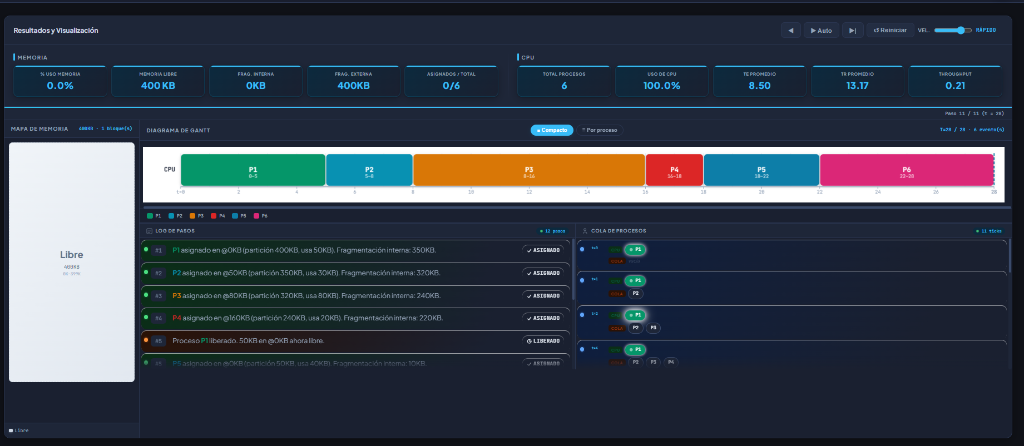
\includegraphics[width=1\linewidth]{figuras/IMAGEN_4.png}
    \caption{Diagrama de Gantt (FCFS)}
    \par\vspace{0.2cm}\raggedright \textit{Nota.} Esta gráfica ilustra la ejecución secuencial bajo el algoritmo FCFS, evidenciando el claro efecto convoy generado por el proceso inicial que acapara la CPU, forzando a los demás a permanecer prolongadamente en estado de espera.
\end{figure}

\begin{table}[H]
\centering\footnotesize
\caption{Resultados Métricos - FCFS}
\begin{tabularx}{\textwidth}{l c c c c c}
\toprule
\textbf{Proceso} & \textbf{Llegada} & \textbf{Ráfaga} & \textbf{T. Espera} & \textbf{T. Retorno} & \textbf{T. Respuesta} \\
\midrule
P1 & 0 & 5 & 0 & 5 & 0 \\
P2 & 1 & 3 & 4 & 7 & 4 \\
P3 & 2 & 8 & 6 & 14 & 6 \\
P4 & 4 & 2 & 12 & 14 & 12 \\
P5 & 5 & 4 & 13 & 17 & 13 \\
P6 & 6 & 6 & 16 & 22 & 16 \\
\midrule
\multicolumn{3}{r}{\textbf{Promedio}} & \textbf{8.50} & \textbf{13.16} & \textbf{8.50} \\
\bottomrule
\end{tabularx}
    \par\vspace{0.2cm}\raggedright \textit{Nota.} Los datos exponen las métricas recopiladas por el algoritmo First-Come, First-Served. Se evidencia una alta penalización temporal reflejada en el tiempo de retorno y respuesta, producto del efecto convoy.
\end{table}

\subsubsection{Algoritmo SJF}
La Figura 4 demuestra la reorganización dinámica de la cola de listos. Al finalizar P1 en $t=7$, el despachador ignora el orden de llegada y prioriza a P3 debido a su ráfaga mínima (1 tick). Esta simple decisión condensa la curva de finalización y recorta el promedio global de espera.
\begin{figure}[H]
    \centering
    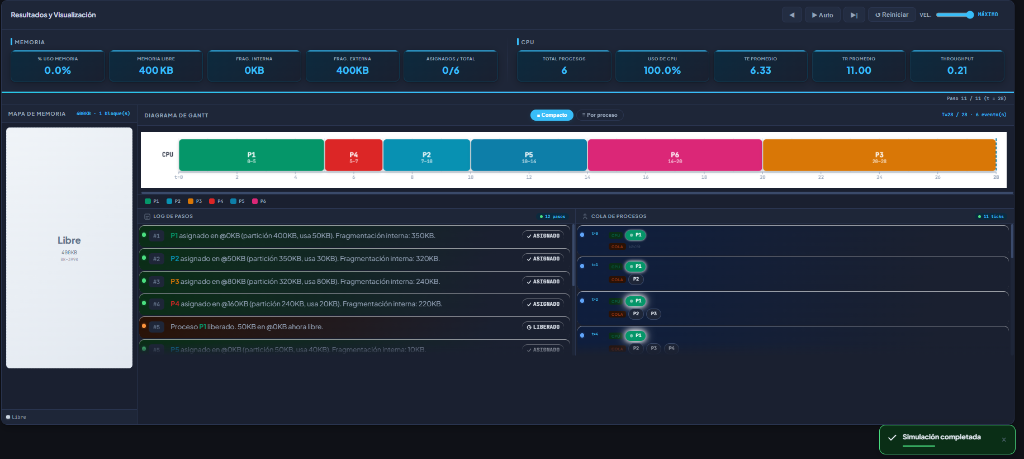
\includegraphics[width=1\linewidth]{figuras/IMAGEN_5.png}
    \caption{Diagrama de Gantt (SJF)}
    \par\vspace{0.2cm}\raggedright \textit{Nota.} Esta figura muestra la reorganización de la cola bajo la política SJF, demostrando cómo la priorización de las ráfagas más cortas minimiza los tiempos de espera promedios frente a las planificaciones secuenciales.
\end{figure}

\begin{table}[H]
\centering\footnotesize
\caption{Resultados Métricos - SJF}
\begin{tabularx}{\textwidth}{l c c c c c}
\toprule
\textbf{Proceso} & \textbf{Llegada} & \textbf{Ráfaga} & \textbf{T. Espera} & \textbf{T. Retorno} & \textbf{T. Respuesta} \\
\midrule
P1 & 0 & 5 & 0 & 5 & 0 \\
P2 & 1 & 3 & 6 & 9 & 6 \\
P3 & 2 & 8 & 18 & 26 & 18 \\
P4 & 4 & 2 & 1 & 3 & 1 \\
P5 & 5 & 4 & 5 & 9 & 5 \\
P6 & 6 & 6 & 8 & 14 & 8 \\
\midrule
\multicolumn{3}{r}{\textbf{Promedio}} & \textbf{6.33} & \textbf{11.00} & \textbf{6.33} \\
\bottomrule
\end{tabularx}
    \par\vspace{0.2cm}\raggedright \textit{Nota.} Esta tabla desglosa el desempeño de Shortest Job First. Los promedios denotan una mejora dramática en la atención global, aunque enmascaran potenciales riesgos de inanición en procesos largos.
\end{table}

\subsubsection{Algoritmo SRT}
La Figura 5 refleja el impacto directo de la expropiación algorítmica. En $t=2$, la llegada de P2 expulsa a P1, y posteriormente en $t=4$, P3 desaloja a P2. Los múltiples cambios de contexto garantizan la atención inmediata de procesos cortos, fragmentando severamente el ciclo de CPU pero optimizando los tiempos de respuesta.
\begin{figure}[H]
    \centering
    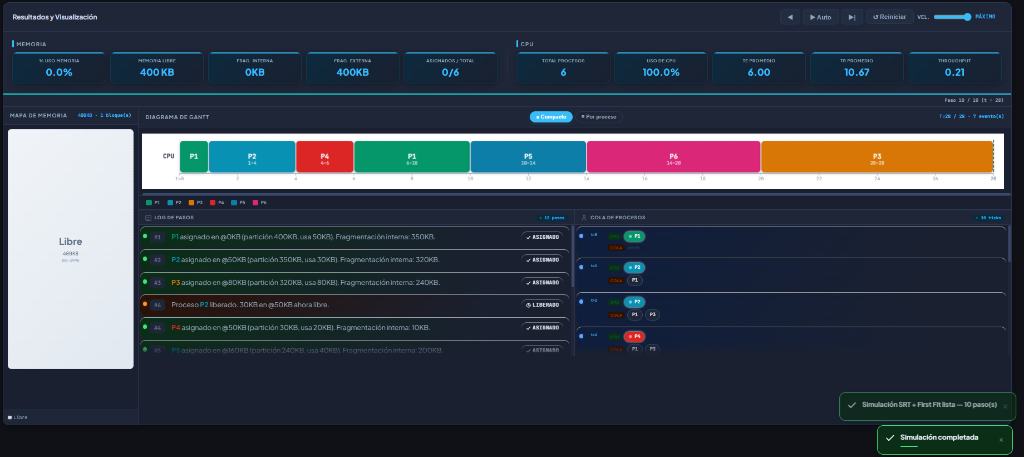
\includegraphics[width=1\linewidth]{figuras/IMAGEN_6.png}
    \caption{Diagrama de Gantt con expropiación (SRT)}
    \par\vspace{0.2cm}\raggedright \textit{Nota.} La ilustración exhibe el comportamiento del planificador SRT, destacando los múltiples cambios de contexto producidos por la apropiación, lo cual permite la atención inmediata de procesos emergentes con menores requerimientos de CPU.
\end{figure}

\begin{table}[H]
\centering\footnotesize
\caption{Resultados Métricos - SRT}
\begin{tabularx}{\textwidth}{l c c c c c}
\toprule
\textbf{Proceso} & \textbf{Llegada} & \textbf{Ráfaga} & \textbf{T. Espera} & \textbf{T. Retorno} & \textbf{T. Respuesta} \\
\midrule
P1 & 0 & 5 & 5 & 10 & 0 \\
P2 & 1 & 3 & 0 & 3 & 0 \\
P3 & 2 & 8 & 18 & 26 & 18 \\
P4 & 4 & 2 & 0 & 2 & 0 \\
P5 & 5 & 4 & 5 & 9 & 5 \\
P6 & 6 & 6 & 8 & 14 & 8 \\
\midrule
\multicolumn{3}{r}{\textbf{Promedio}} & \textbf{6.00} & \textbf{10.66} & \textbf{5.16} \\
\bottomrule
\end{tabularx}
    \par\vspace{0.2cm}\raggedright \textit{Nota.} Los indicadores demuestran la superioridad del modelo expulsivo SRT en los tiempos de respuesta. Las interrupciones oportunas minimizan las esperas iniciales frente a la competencia de tareas cortas.
\end{table}

\subsubsection{Algoritmo Round Robin (Quantum = 2)}
La Figura 6 evidencia la multiplexación temporal estricta. El temporizador simula cortes forzados cada 2 ticks, obligando a procesos pesados como P3 (8 ms) a ceder la CPU repetidas veces para que el resto pueda avanzar. Aunque esto eleva la espera general, asegura una interactividad equitativa que previene la inanición absoluta.
\begin{figure}[H]
    \centering
    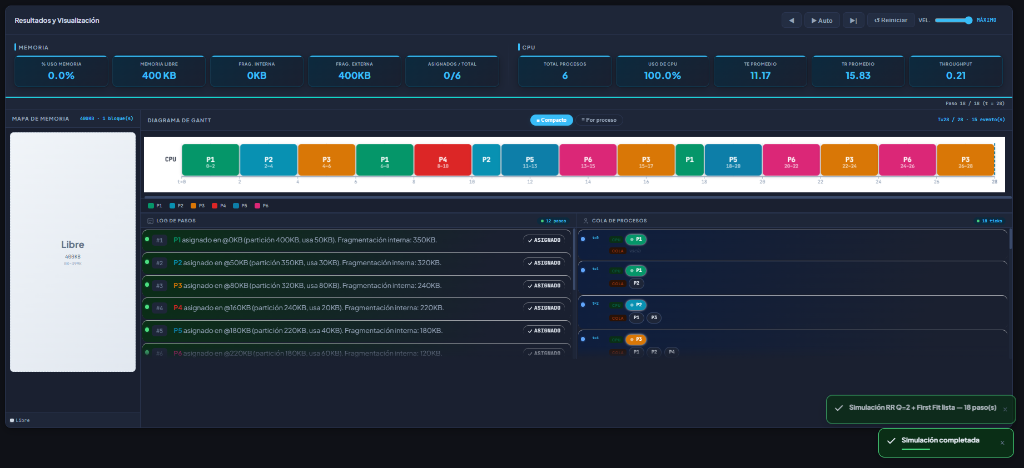
\includegraphics[width=1\linewidth]{figuras/IMAGEN_7.png}
    \caption{Diagrama de Gantt segmentado por Quantum (RR)}
    \par\vspace{0.2cm}\raggedright \textit{Nota.} El diagrama evidencia la multiplexación temporal impuesta por el algoritmo Round Robin, donde los cortes por quántum fuerzan una rotación cíclica equitativa entre los procesos concurrentes.
\end{figure}

\begin{table}[H]
\centering\footnotesize
\caption{Resultados Métricos - Round Robin}
\begin{tabularx}{\textwidth}{l c c c c c}
\toprule
\textbf{Proceso} & \textbf{Llegada} & \textbf{Ráfaga} & \textbf{T. Espera} & \textbf{T. Retorno} & \textbf{T. Respuesta} \\
\midrule
P1 & 0 & 5 & 13 & 18 & 0 \\
P2 & 1 & 3 & 7 & 10 & 1 \\
P3 & 2 & 8 & 18 & 26 & 2 \\
P4 & 4 & 2 & 4 & 6 & 4 \\
P5 & 5 & 4 & 11 & 15 & 6 \\
P6 & 6 & 6 & 14 & 20 & 7 \\
\bottomrule
\end{tabularx}
    \par\vspace{0.2cm}\raggedright \textit{Nota.} La tabla cuantifica la rotación cíclica controlada por el quántum. Aunque el tiempo de retorno se alarga por los constantes cambios de contexto, la equidad de respuesta queda plenamente garantizada.
\end{table}

\subsection{Resultados Memoria}
Para someter a estrés las políticas de asignación, el sistema delimita 1024 KB de RAM total y reserva 100 KB bloqueados para el Sistema Operativo. Se inyectan de forma secuencial los 6 procesos del escenario base, los cuales demandan un total de 280 KB. Debido a que el espacio libre inicial (924 KB) es holgadamente superior a la demanda, las políticas de partición dinámica (First Fit y Best Fit) operan idénticamente en la primera pasada, asignando la memoria de manera contigua sin provocar fragmentación externa en los bloques instanciados.

\begin{figure}[H]
    \centering
    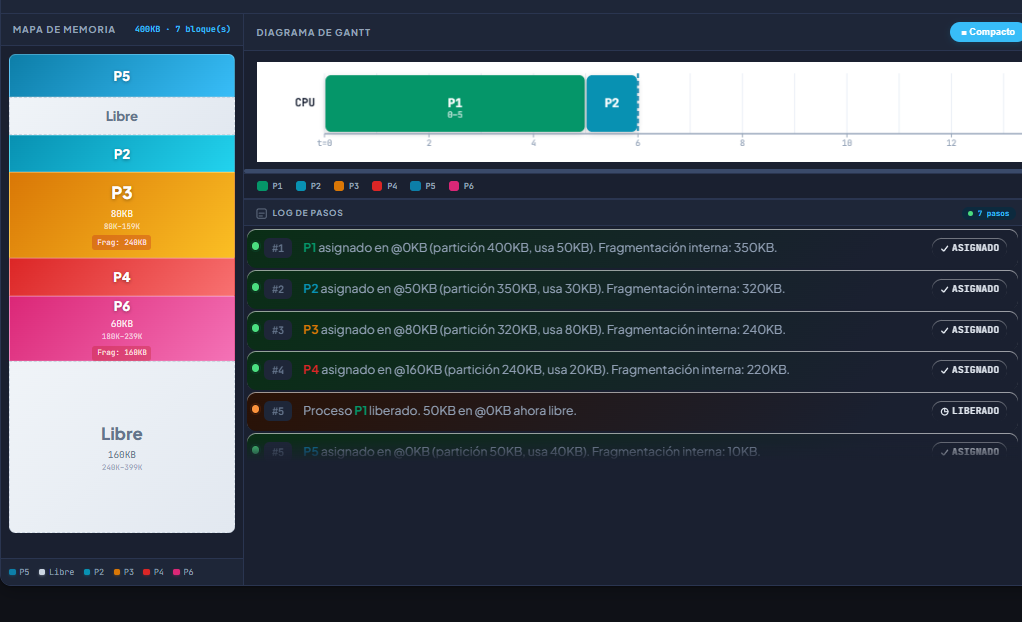
\includegraphics[width=1\linewidth]{figuras/IMAGEN_8.png}
    \caption{Mapa de Memoria (Particionamiento Dinámico Secuencial)}
    \par\vspace{0.2cm}\raggedright \textit{Nota.} La figura despliega el mapa espacial resultante de la partición dinámica, donde los bloques son asignados consecutivamente según la política First/Best Fit debido a la holgura inicial, evitando momentáneamente la fragmentación externa.
\end{figure}

\begin{table}[H]
\centering\footnotesize
\caption{Tabla de Asignación - Partición Dinámica (First / Best Fit)}
\begin{tabularx}{\textwidth}{l c c c c c}
\toprule
\textbf{Bloque} & \textbf{Tamaño Sol.} & \textbf{Partición Asignada} & \textbf{Dir. Inicio} & \textbf{Dir. Fin} & \textbf{Frag. Interna} \\
\midrule
SO & - & 100 KB & 0 KB & 99 KB & 0 KB \\
P1 & 50 KB & 50 KB & 100 KB & 149 KB & 0 KB \\
P2 & 30 KB & 30 KB & 150 KB & 179 KB & 0 KB \\
P3 & 80 KB & 80 KB & 180 KB & 259 KB & 0 KB \\
P4 & 20 KB & 20 KB & 260 KB & 279 KB & 0 KB \\
P5 & 40 KB & 40 KB & 280 KB & 319 KB & 0 KB \\
P6 & 60 KB & 60 KB & 320 KB & 379 KB & 0 KB \\
Libre & - & 644 KB & 380 KB & 1023 KB & 0 KB \\
\bottomrule
\end{tabularx}
    \par\vspace{0.2cm}\raggedright \textit{Nota.} Esta tabla desglosa las ubicaciones exactas de cada proceso en RAM bajo un modelo dinámico. Se constata el nulo desperdicio interno debido a que los límites de cada bloque se ajustan milimétricamente al tamaño exigido.
\end{table}

Sin embargo, la Figura 8 revela la drástica reorganización celular impuesta por el Buddy System frente a la misma carga de 280 KB. Al restringir las particiones a potencias exactas de 2, la interfaz segmenta visualmente las zonas obligando a cada proceso a encajar en un bloque geométricamente rígido. El análisis matemático corrobora un desperdicio inmediato: los 6 procesos ocupan un total de 384 KB en la RAM, generando 104 KB de pura fragmentación interna.

\begin{figure}[H]
    \centering
    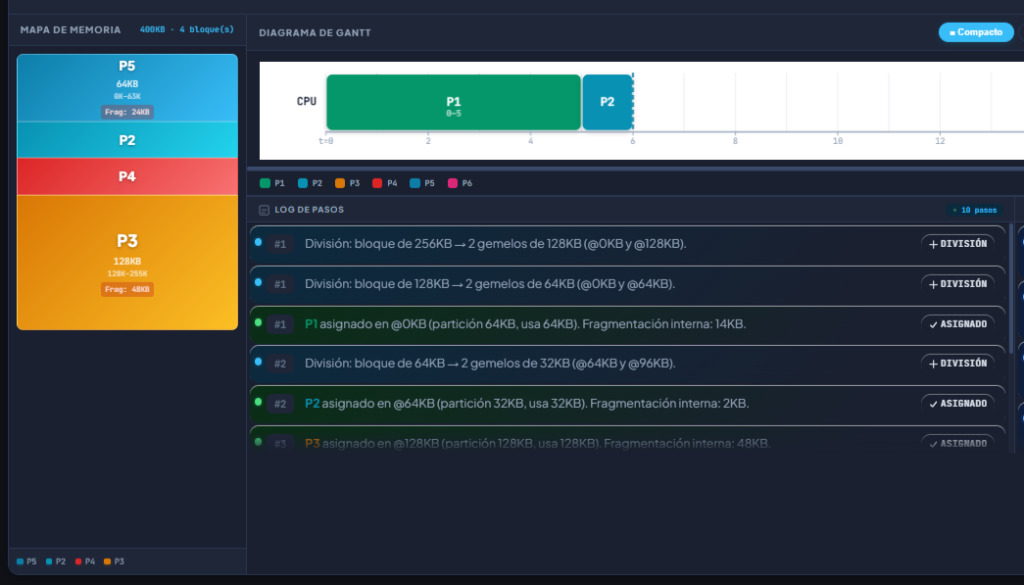
\includegraphics[width=1\linewidth]{figuras/IMAGEN_9.png}
    \caption{Mapa particionado en potencias de 2 (Buddy System)}
    \par\vspace{0.2cm}\raggedright \textit{Nota.} El esquema visualiza la estricta alineación geométrica del sistema colega. La partición top-down encuadra cada requerimiento dentro del bloque de potencia de 2 más cercano, causando fragmentación interna apreciable.
\end{figure}

\begin{table}[H]
\centering\footnotesize
\caption{Análisis de Fragmentación Interna - Buddy System}
\begin{tabularx}{\textwidth}{l c c c c}
\toprule
\textbf{Proceso} & \textbf{Tamaño Sol.} & \textbf{Bloque Asignado (2\textsuperscript{n})} & \textbf{Memoria Desperdiciada} \\
\midrule
P1 & 50 KB & 64 KB & 14 KB \\
P2 & 30 KB & 32 KB & 2 KB \\
P3 & 80 KB & 128 KB & 48 KB \\
P4 & 20 KB & 32 KB & 12 KB \\
P5 & 40 KB & 64 KB & 24 KB \\
P6 & 60 KB & 64 KB & 4 KB \\
\midrule
\multicolumn{3}{r}{\textbf{Total de Fragmentación Interna:}} & \textbf{104 KB} \\
\bottomrule
\end{tabularx}
    \par\vspace{0.2cm}\raggedright \textit{Nota.} La tabla cuantifica directamente el desperdicio espacial inherente al sistema colega. El redondeo forzoso hacia la potencia de dos más cercana provoca una suma considerable de fragmentos inútiles.
\end{table}

\subsection{Resultados de Almacenamiento Secundario (Disco)}
El motor de almacenamiento fue sometido a cargas de escritura progresivas para probar la viabilidad espacial de sus 7 esquemas algorítmicos. Para gestionar las operaciones de entrada/salida y la localización física de la información, el núcleo simula en memoria principal una \textbf{Tabla de Directorio (Metadatos)}. Dado que la estructura de esta tabla varía drásticamente dependiendo del algoritmo de asignación evaluado, se detalla su comportamiento estructural bajo cada esquema, tomando como referencia los archivos base \texttt{SISTEMA} y \texttt{KERNEL}.

\subsubsection{Asignación Contigua}
La Figura 9 grafica el modelo en su forma más pura. La contigüidad absoluta facilita lecturas íntegras a máxima velocidad, pero detona colisiones irreversibles. Al intentar expandir un archivo en tiempo de ejecución, el bloque colindante ocupado desencadena un fallo de asignación, requiriendo compactación mecánica del disco.
\begin{figure}[H]
    \centering
    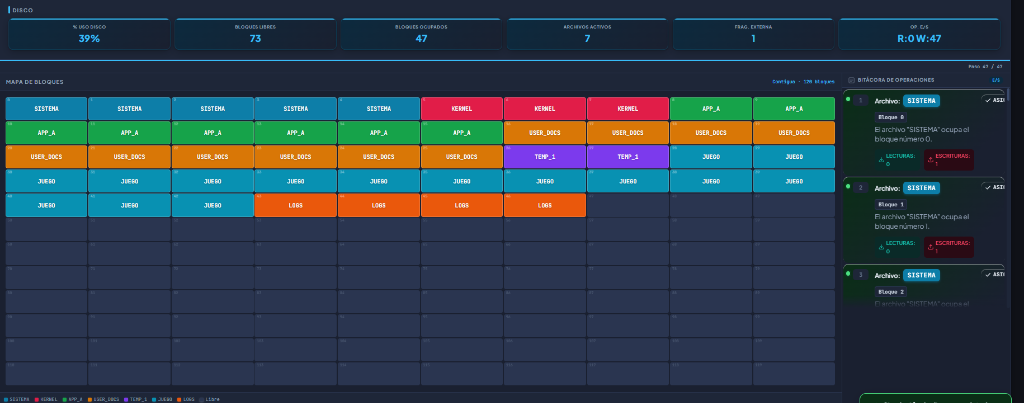
\includegraphics[width=1\linewidth]{figuras/IMAGEN_11.png}
    \caption{Mapa de clústeres contiguos demostrando fragmentación externa (Disco)}
    \par\vspace{0.2cm}\raggedright \textit{Nota.} La figura expone la asignación contigua en el almacenamiento secundario, ilustrando la vulnerabilidad estructural ante expansiones y el riesgo inminente de fragmentación externa masiva.
\end{figure}

\begin{table}[H]
\centering\footnotesize
\caption{Estructura del Directorio - Asignación Contigua}
\begin{tabularx}{0.6\textwidth}{l c c}
\toprule
\textbf{Archivo} & \textbf{Bloque Inicio} & \textbf{Longitud} \\
\midrule
SISTEMA & 0 & 5 \\
KERNEL & 5 & 3 \\
\bottomrule
\end{tabularx}
    \par\vspace{0.2cm}\raggedright \textit{Nota.} Los datos detallan los metadatos almacenados en memoria principal para el algoritmo contiguo, donde cada archivo es rastreado únicamente mediante su bloque inicial lógico y la cantidad total de bloques.
\end{table}

\subsubsection{Asignación Enlazada}
La Figura 10 plasma la superación física de las fronteras de contigüidad. Los archivos se dispersan erráticamente a lo largo del grid del disco, reconectándose a través de punteros intra-bloque. La interfaz demuestra gráficamente la penalización: la pérdida de 4 bytes efectivos por bloque infla directamente el Overhead operativo del sistema.
\begin{figure}[H]
    \centering
    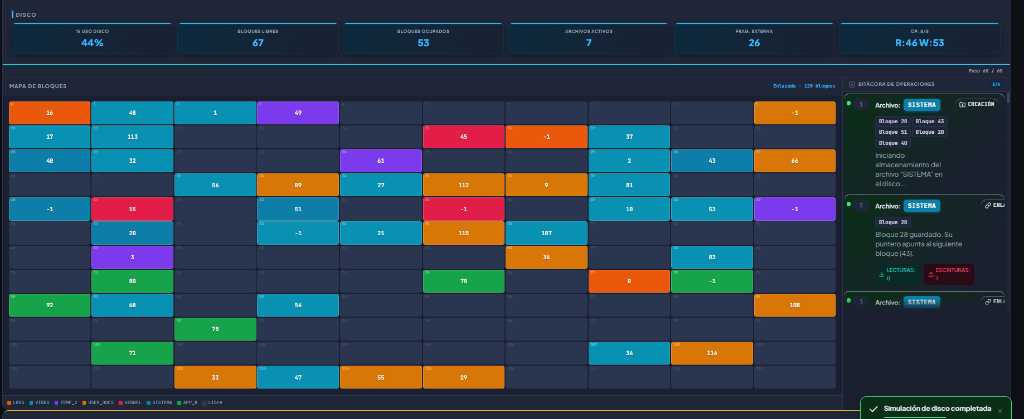
\includegraphics[width=1\linewidth]{figuras/IMAGEN_12.png}
    \caption{Trazabilidad visual de punteros intrabloque (Asignación Enlazada)}
    \par\vspace{0.2cm}\raggedright \textit{Nota.} Este mapa traza el enlazamiento de clústeres dispersos a través del disco. La dispersión espacial elimina la fragmentación externa, penalizando sin embargo las lecturas aleatorias a causa de saltos mecánicos.
\end{figure}

\begin{table}[H]
\centering\footnotesize
\caption{Estructura del Directorio - Asignación Enlazada}
\begin{tabularx}{0.6\textwidth}{l c c}
\toprule
\textbf{Archivo} & \textbf{Bloque Inicio} & \textbf{Bloque Fin} \\
\midrule
SISTEMA & 28 & 43 \\
KERNEL & 15 & 71 \\
\bottomrule
\end{tabularx}
    \par\vspace{0.2cm}\raggedright \textit{Nota.} La tabla exhibe la información mínima registrada por el directorio bajo el esquema de enlaces, almacenando sólo los nodos de cabecera y terminación de la cadena secuencial en el disco.
\end{table}

\subsubsection{Asignación Indexada}
La Figura 11 exhibe la centralización del mapeo. El bloque primario muta en un nodo índice que ramifica el control hacia los bloques de datos esparcidos. Se certifica visualmente el desperdicio inherente: un archivo que apenas ocupa 1 bloque de datos exige forzosamente el sacrificio de 1 bloque entero para indexación estructural.
\begin{figure}[H]
    \centering
    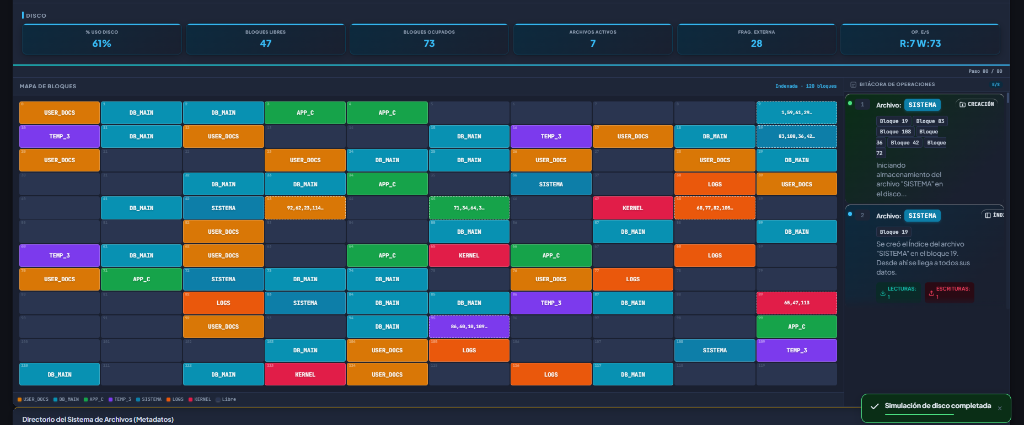
\includegraphics[width=1\linewidth]{figuras/IMAGEN_13.png}
    \caption{Bloque índice centralizando las direcciones de datos (Indexada Simple)}
    \par\vspace{0.2cm}\raggedright \textit{Nota.} La imagen muestra el mapeo centralizado donde un nodo índice asume el control posicional, garantizando acceso directo a expensas de sacrificar bloques íntegros exclusivos para los metadatos.
\end{figure}

\begin{table}[H]
\centering\footnotesize
\caption{Estructura del Directorio - Indexada Simple}
\begin{tabularx}{0.6\textwidth}{l c}
\toprule
\textbf{Archivo} & \textbf{Bloque Índice Principal} \\
\midrule
SISTEMA & 19 \\
KERNEL & 133 \\
\bottomrule
\end{tabularx}
    \par\vspace{0.2cm}\raggedright \textit{Nota.} Esta tabla denota cómo el directorio remite la gestión posicional de cada archivo a un único bloque índice, que encapsula las coordenadas precisas de toda la estructura subyacente.
\end{table}

\subsubsection{Tabla de Asignación de Archivos (FAT)}
La Figura 12 presenta el desplazamiento del control hacia la RAM. La tabla virtual mapea cadenas enlazadas sin consumir un solo byte dentro del plato magnético de datos. El simulador erradica las lecturas redundantes, reflejando accesos mucho más livianos e íntegros frente al esquema de enlazado clásico.
\begin{figure}[H]
    \centering
    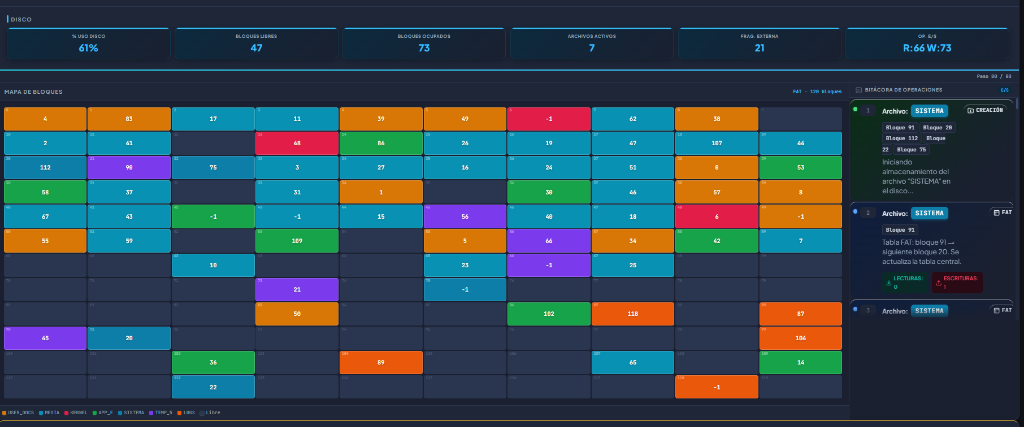
\includegraphics[width=1\linewidth]{figuras/IMAGEN_14.png}
    \caption{Estructura tabular de enlazamiento replicando la FAT en RAM}
    \par\vspace{0.2cm}\raggedright \textit{Nota.} Esta ilustración representa la tabla FAT instanciada en memoria principal, exponiendo cómo el redireccionamiento lógico evita la lectura secuencial de sectores magnéticos e incrementa la velocidad general.
\end{figure}

\begin{table}[H]
\centering\footnotesize
\caption{Estructura del Directorio - FAT}
\begin{tabularx}{0.6\textwidth}{l c}
\toprule
\textbf{Archivo} & \textbf{Bloque de Inicio} \\
\midrule
SISTEMA & 91 \\
KERNEL & 48 \\
\bottomrule
\end{tabularx}
    \par\vspace{0.2cm}\raggedright \textit{Nota.} Los registros revelan el vínculo inicial apuntado por el directorio para consultar la File Allocation Table, un método que traslada el recorrido exhaustivo de enlaces hacia la Memoria RAM.
\end{table}

\subsubsection{Indexada Multinivel (Estilo UNIX)}
La Figura 13 prueba la escalabilidad asintótica. Al simular la inyección de un fichero masivo que satura el bloque índice inicial, el sistema escala instanciando dinámicamente apuntadores de segundo y tercer nivel, validando el núcleo conceptual de los inodos bajo condiciones de desbordamiento de metadatos.
\begin{figure}[H]
    \centering
    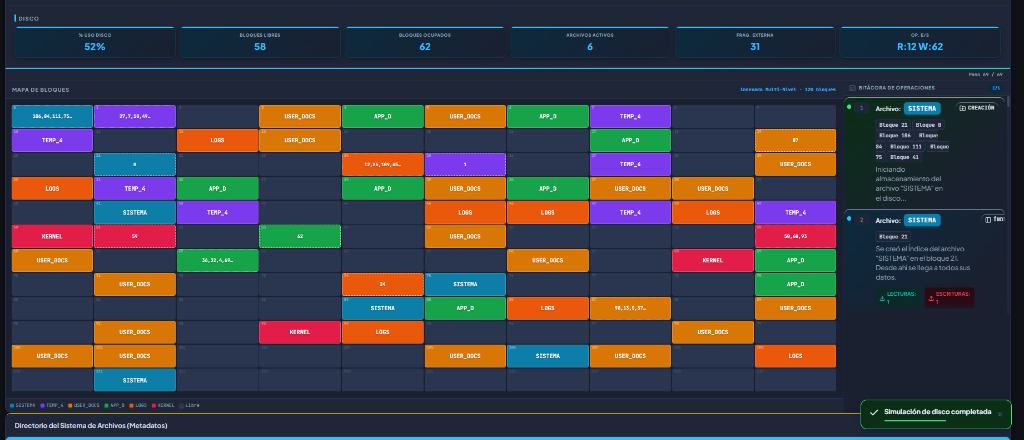
\includegraphics[width=1\linewidth]{figuras/IMAGEN_15.png}
    \caption{Estructura jerárquica de índices (Asignación Multinivel)}
    \par\vspace{0.2cm}\raggedright \textit{Nota.} El gráfico despliega el escalamiento en árbol característico del modelo UNIX, con índices primarios que apuntan a secundarios frente al desbordamiento ocasionado por ficheros de envergadura masiva.
\end{figure}

\begin{table}[H]
\centering\footnotesize
\caption{Estructura del Directorio - Indexada Multinivel}
\begin{tabularx}{0.6\textwidth}{l c}
\toprule
\textbf{Archivo} & \textbf{Índice Primario (Nivel 1)} \\
\midrule
SISTEMA & 21 \\
KERNEL & 59 \\
\bottomrule
\end{tabularx}
    \par\vspace{0.2cm}\raggedright \textit{Nota.} La tabla muestra la dirección de los índices primarios raíz, los cuales actúan como la entrada principal de un árbol jerárquico multinivel ideado para gestionar metadatos de archivos grandes.
\end{table}

\subsubsection{Asignación por Extensiones (Extents)}
La Figura 14 revela una compresión de metadatos drástica. En lugar de registrar un centenar de punteros para un fichero contiguo de 100 bloques, la matriz del sistema condensa todo el rastreo lógico en una única tupla geométrica que delimita el inicio del recorrido y su salto espacial.
\begin{figure}[H]
    \centering
    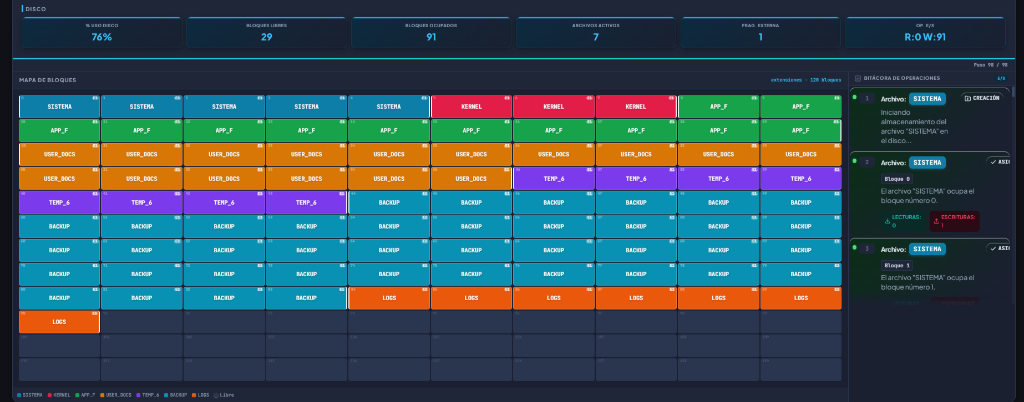
\includegraphics[width=1\linewidth]{figuras/IMAGEN_16.png}
    \caption{Compresión de punteros mediante Extents}
    \par\vspace{0.2cm}\raggedright \textit{Nota.} La figura demuestra la asignación basada en extensiones, confirmando cómo una vasta cantidad de sectores continuos son referenciados de manera óptima por una sola tupla que marca inicio y tamaño.
\end{figure}

\begin{table}[H]
\centering\footnotesize
\caption{Estructura del Directorio - Extensiones (Extents)}
\begin{tabularx}{0.6\textwidth}{l c}
\toprule
\textbf{Archivo} & \textbf{Tupla (Inicio, Longitud)} \\
\midrule
SISTEMA & (0, 5) \\
KERNEL & (5, 3) \\
\bottomrule
\end{tabularx}
    \par\vspace{0.2cm}\raggedright \textit{Nota.} Este registro ilustra la máxima simplificación del rastreo. Se detalla la condensación geométrica en tuplas que agrupan secuencias contiguas reduciendo el peso de la información administrativa.
\end{table}

\subsubsection{Gestión por Mapa de Bits (Bitmap)}
La Figura 15 mapea visualmente el estado libre y ocupado del disco mediante renderizado binario estricto. La búsqueda de espacios vacíos muta hacia una simple exploración matemática, garantizando recuperaciones y asignaciones aceleradas sin intervenir bloques de datos físicamente.
\begin{figure}[H]
    \centering
    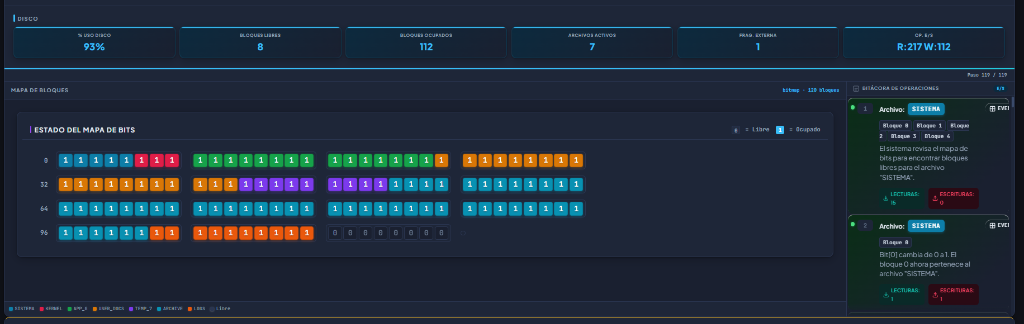
\includegraphics[width=1\linewidth]{figuras/IMAGEN_17.png}
    \caption{Mapeo binario de sectores ocupados (Bitmap)}
    \par\vspace{0.2cm}\raggedright \textit{Nota.} La visualización evidencia el control de almacenamiento sustentado en arreglos de bits, un esquema de alta velocidad matemática diseñado para descubrir rangos vacíos sin examinar físicamente los platos.
\end{figure}

\begin{table}[H]
\centering\footnotesize
\caption{Estructura del Directorio - Mapa de Bits}
\begin{tabularx}{0.6\textwidth}{l c c}
\toprule
\textbf{Archivo} & \textbf{Bloque Inicio} & \textbf{Longitud} \\
\midrule
SISTEMA & 8 & 5 \\
KERNEL & 13 & 3 \\
\bottomrule
\end{tabularx}
    \par\vspace{0.2cm}\raggedright \textit{Nota.} La tabla evidencia la persistencia del archivo basada en el mapeo inicial, el cual debe contrastarse posteriormente contra el arreglo binario del disco para localizar los flujos libres adyacentes.
\end{table}

Como consolidación de los ensayos en el Almacenamiento Secundario, la siguiente tabla extrae las métricas globales de ejecución registradas durante las simulaciones. Estos datos evidencian empíricamente la compensación directa entre la eficiencia espacial (reducción de fragmentación externa) y el coste administrativo de los metadatos (operaciones de Lectura/Escritura):

\begin{table}[H]
\centering\footnotesize
\caption{Resultados Métricos Consolidados - Algoritmos de Disco}
\begin{tabularx}{\textwidth}{l c c c c c}
\toprule
\textbf{Algoritmo} & \textbf{Uso de Disco} & \textbf{Bloques Ocupados} & \textbf{Frag. Externa} & \textbf{Op. Lectura} & \textbf{Op. Escritura} \\
\midrule
Contigua & 39\% & 47 & 1 & 0 & 47 \\
Enlazada & 44\% & 53 & 26 & 46 & 53 \\
Indexada Simple & 61\% & 73 & 28 & 7 & 73 \\
FAT & 61\% & 73 & 21 & 66 & 73 \\
Indexada Multinivel & 52\% & 62 & 31 & 12 & 62 \\
Extensiones (Extents) & 76\% & 91 & 1 & 0 & 91 \\
Mapa de Bits (Bitmap) & 93\% & 112 & 1 & 217 & 112 \\
\bottomrule
\end{tabularx}
    \par\vspace{0.2cm}\raggedright \textit{Nota.} La tabla consolida el rendimiento comparado entre múltiples enfoques, revelando empíricamente la tensión ineludible entre un eficiente acceso espacial y el costo volumétrico de los metadatos requeridos.
\end{table}

% ==========================================
% 7. ANÁLISIS DE RENDIMIENTO COMPARATIVO
% ==========================================
\section{Análisis de Rendimiento Comparativo}

\subsection{Procesador (CPU)}
La evaluación de los cuatro planificadores expone contrastes agudos en el manejo del tiempo. Como se evidenció en los resultados, FCFS penaliza severamente los tiempos de espera cuando procesos largos monopolizan el procesador, provocando un tiempo de espera promedio de 8.50 ms en el escenario de prueba. Por el contrario, SJF optimizó este valor a 6.33 ms al priorizar ráfagas cortas, aunque exige conocer el tiempo de ejecución por adelantado. La introducción de la expropiación en SRT redujo aún más la espera a 6.00 ms, demostrando ser matemáticamente superior para sistemas reactivos, pero incurriendo en un alto número de cambios de contexto. Finalmente, Round Robin (Quantum = 2) sacrificó el tiempo de retorno (elevándolo a 15.83 ms) a cambio de garantizar equidad e interactividad, rotando los procesos cíclicamente sin permitir inanición.

\begin{table}[H]
\centering\small
\caption{Consolidado de algoritmos de planificación de CPU}
\label{tab:comp_cpu}
\begin{tabularx}{\textwidth}{X c c c X}
\toprule
\textbf{Algoritmo} & \textbf{Expulsivo} & \textbf{Overhead} & \textbf{T. Espera} & \textbf{Aplicabilidad} \\
\midrule
FCFS & No & Bajo & Alto & Batch simple \\
SJF & No & Bajo & Óptimo & Bach predecible \\
SRT & Sí & Alto & Muy Bajo & Batch iterativo interactivo \\
RR & Sí & Medio & Moderado & Entornos multiprogramados \\
\bottomrule
\end{tabularx}
    \par\vspace{0.2cm}\raggedright \textit{Nota.} Esta tabla compendia la evaluación final de los planificadores. Se contrastan los costos de contexto (overhead), las políticas de expulsión y los nichos de aplicabilidad en los sistemas modernos.
\end{table}

\subsection{Memoria Principal}
El contraste empírico entre las estrategias de particionamiento continuo y el sistema de colegas subraya un intercambio directo entre tipos de fragmentación. Las políticas de First Fit y Best Fit lograron evadir la fragmentación interna por completo, asignando bloques exactos a la medida de los procesos. Sin embargo, este diseño es altamente propenso a fragmentación externa a medida que los procesos terminan y dejan huecos esparcidos. En contraparte, el algoritmo Buddy System resolvió la gestión de la memoria de forma radicalmente distinta: al restringir los bloques a potencias exactas de 2, el mapa de memoria acomodó 280 KB de procesos dentro de 384 KB de RAM, generando 104 KB de fragmentación interna. Pese a este desperdicio inmediato, la arquitectura rígida de potencias facilita una coalescencia acelerada, demostrando por qué sigue siendo la estrategia predilecta en el núcleo de sistemas robustos como Linux.

\begin{table}[H]
\centering\small
\caption{Consolidado de algoritmos de Gestión de Memoria}
\label{tab:comp_mem}
\begin{tabularx}{\textwidth}{X c c c X}
\toprule
\textbf{Algoritmo} & \textbf{Velocidad Búsqueda} & \textbf{Frag. Externa} & \textbf{Frag. Interna} & \textbf{Observación Clave} \\
\midrule
First Fit & Muy Rápida & Alta a largo plazo & Nula & Concentra carga al inicio \\
Best Fit & Lenta (Búsqueda total) & Muy Alta (Astillas) & Nula & Teóricamente ideal, prácticamente deficiente \\
Worst Fit & Lenta / Ordenada & Moderada & Nula & Genera huecos residuales usables \\
Buddy System & Rápida (Árbol 2\textsuperscript{k}) & Muy Baja & Alta & Coalescencia ultrarrápida, ideal en kernels \\
\bottomrule
\end{tabularx}
    \par\vspace{0.2cm}\raggedright \textit{Nota.} Este resumen coteja la balanza de fragmentación de las estrategias en RAM. Exalta la eficiencia del particionamiento matemático top-down frente al análisis exhaustivo y costoso del Best Fit.
\end{table}

\subsection{Almacenamiento Secundario (Disco)}
El módulo de disco comprobó de primera mano las abismales diferencias operativas entre los siete paradigmas de asignación. La estructura contigua logró evitar por completo las lecturas dispersas, pero chocó de frente con la fragmentación externa (fallando críticamente al intentar expandir un archivo). Las arquitecturas enlazadas e indexadas solucionaron esta limitación física, pero los logs del sistema arrojaron un costo altísimo en operaciones de E/S; por ejemplo, el índice multinivel y la estructura FAT exigieron ráfagas masivas de escritura tan solo para enlazar metadatos. Frente a estas deficiencias mecánicas, modelos híbridos como las Extensiones (Extents) probaron su supremacía, logrando comprimir cientos de punteros lógicos en una sola tupla geométrica. De igual forma, el Mapa de Bits (Bitmap) evidenció la vía más veloz para localizar espacios libres, al rasterizar el volumen del disco en simples matrices de ceros y unos procesables matemáticamente.

\begin{table}[H]
\centering\small
\caption{Consolidado de algoritmos de Gestión de Disco}
\label{tab:comp_disco}
\begin{tabularx}{\textwidth}{X c c c X}
\toprule
\textbf{Algoritmo} & \textbf{Acceso Directo} & \textbf{Frag. Externa} & \textbf{Overhead ($O_d$)} & \textbf{Expansión Archivo} \\
\midrule
Contigua & Excelente ($O(1)$) & Severa & Mínimo & Extremadamente Difícil \\
Enlazada & Nulo ($O(N)$) & Nula & Alto & Muy Fácil \\
Indexada & Excelente ($O(1)$) & Nula & Muy Alto & Limitado al índice \\
FAT & Excelente (en RAM) & Nula & Moderado (Central) & Fácil \\
Multinivel & Excelente & Nula & Dinámico & Óptimo para gigantes \\
Extents & Excelente & Baja (si es contiguo) & Ultrabajo & Fácil y eficiente \\
\bottomrule
\end{tabularx}
    \par\vspace{0.2cm}\raggedright \textit{Nota.} La tabla sintetiza las fortalezas estructurales y deficiencias algorítmicas al almacenar datos a largo plazo, confirmando la evolución hacia modelos compuestos que mitigaron limitaciones de la contigüidad pura.
\end{table}

\subsection{Sinergia del Sistema Integral}
La evaluación aislada de cada componente consolida una métrica final sobre el comportamiento global del núcleo. Un planificador de CPU ultrarrápido (SRT) pierde toda efectividad si la memoria principal padece fragmentación externa severa (First Fit) que retrase la inyección de procesos. De igual forma, una gestión de RAM impecable (Buddy System) colapsará el rendimiento general si el almacenamiento secundario incurre en operaciones mecánicas excesivas (Asignación Enlazada). Los resultados empíricos obtenidos demuestran que la arquitectura de un sistema operativo moderno no se optimiza maximizando el rendimiento de un solo módulo, sino estructurando una sinergia operativa donde las deficiencias matemáticas de un algoritmo son mitigadas directamente por las fortalezas de la capa adyacente.

% ==========================================
% 8. CONCLUSIONES
% ==========================================
\section{Conclusiones}

La evaluación empírica de los algoritmos del núcleo del sistema operativo confirma matemáticamente la premisa central de la ingeniería de sistemas: no existe una política de administración de recursos universalmente superior, sino un delicado balance de compensaciones técnicas entre tiempo de respuesta, fragmentación espacial y desgaste electromecánico. A nivel del procesador, los resultados aislaron los compromisos inherentes a cada planificador; mientras esquemas secuenciales como FCFS sucumben ante el efecto convoy elevando drásticamente la penalización de espera media (8.50 ms), las políticas expropiativas garantizan una optimización asimétrica. Se comprobó que el enfoque Shortest Remaining Time minimiza estadísticamente los tiempos de retorno (6.00 ms) a costa de saturar el sistema con cambios de contexto, en contraste directo con Round Robin, que sacrifica el rendimiento bruto temporal (15.83 ms) para asegurar una multiplexación puramente interactiva y equitativa.

En lo que respecta a la gestión de memoria principal, la simulación de particionamiento dinámico evidenció la incompatibilidad estructural entre la contigüidad absoluta y la prevención de huecos de asignación. Estrategias voraces como First Fit previenen el desperdicio interno, pero decaen inexorablemente frente a la fragmentación externa conforme se liberan bloques aislados. Como contraparte, la implementación matemática del Buddy System demostró la supremacía de la restricción geométrica; al someter los bloques a potencias exactas de dos, el sistema asume de forma deliberada una alta fragmentación interna (104 KB calculados) como el precio algorítmico necesario para erradicar la dispersión externa y habilitar una coalescencia ultrarrápida a nivel de árbol binario.

Finalmente, el análisis métrico sobre el almacenamiento secundario ratificó las limitantes físicas del diseño magnético frente al acceso aleatorio impuesto por los procesos concurrentes. Se verificó que las estructuras primitivas, como la asignación contigua pura y el esquema simplemente enlazado, colapsan irremediablemente ante el crecimiento dinámico de los datos, exigiendo compactaciones mecánicas o generando latencias severas por lecturas intrabloque. En respuesta a esto, las arquitecturas lógicas híbridas como la jerarquía indexada multinivel y la agrupación por extensiones (Extents) probaron ser el punto de convergencia óptimo, logrando comprimir abstracciones de miles de punteros en metadatos ligeros, reduciendo exponencialmente las operaciones de entrada y salida, y garantizando la viabilidad temporal del almacenamiento de alto rendimiento.

\newpage
% ==========================================
% 9. REFERENCIAS
% ==========================================
\section*{Referencias}
\addcontentsline{toc}{section}{Referencias}

\noindent Arpaci-Dusseau, R. H., \& Arpaci-Dusseau, A. C. (2018). \textit{Operating Systems: Three Easy Pieces}. Arpaci-Dusseau Books. \url{https://pages.cs.wisc.edu/~remzi/OSTEP/}

\vspace{0.3cm}
\noindent Corbató, F. J. (1962). An Experimental Time-Sharing System. \textit{Proceedings of the AFIPS Spring Joint Computer Conference}, 335-344. \url{https://doi.org/10.1145/1460833.1460871}

\vspace{0.3cm}
\noindent Denning, P. J. (1970). Virtual Memory. \textit{ACM Computing Surveys}, 2(3), 153-189. \url{https://doi.org/10.1145/356571.356573}

\vspace{0.3cm}
\noindent Knuth, D. E. (1997). \textit{The Art of Computer Programming, Volume 1: Fundamental Algorithms} (3a ed.). Addison-Wesley Professional.

\vspace{0.3cm}
\noindent Love, R. (2010). \textit{Linux Kernel Development} (3a ed.). Addison-Wesley Professional.

\vspace{0.3cm}
\noindent Mathur, A., Cao, M., Bhattacharya, S., Dilger, A., Tomas, A., \& Vivier, L. (2007). The new ext4 filesystem: current status and future plans. \textit{Proceedings of the Linux Symposium}, 2, 21-33. \url{https://www.kernel.org/doc/ols/2007/ols2007v2-pages-21-34.pdf}

\vspace{0.3cm}
\noindent McKusick, M. K., Joy, W. N., Leffler, S. J., \& Fabry, R. S. (1984). A Fast File System for UNIX. \textit{ACM Transactions on Computer Systems}, 2(3), 181-197. \url{https://doi.org/10.1145/989.990}

\vspace{0.3cm}
\noindent Silberschatz, A., Galvin, P. B., \& Gagne, G. (2018). \textit{Operating System Concepts} (10a ed.). Wiley.

\vspace{0.3cm}
\noindent Stallings, W. (2018). \textit{Operating Systems: Internals and Design Principles} (9a ed.). Pearson.

\vspace{0.3cm}
\noindent Tanenbaum, A. S., \& Bos, H. (2015). \textit{Modern Operating Systems} (4a ed.). Pearson.

% ==========================================
% 10. ANEXOS
% ==========================================
\newpage
\section*{Anexos}
\addcontentsline{toc}{section}{Anexos}

\subsection*{A. Repositorio del Código Fuente}
El código fuente íntegro de este simulador interactivo, estructurado modularmente en HTML5, Vanilla CSS y algoritmos en JavaScript puro, ha sido desplegado de forma pública. Para auditar la lógica matemática, inspeccionar la arquitectura del Canvas o probar el proyecto en un entorno de desarrollo local, puede acceder al repositorio oficial de GitHub a través del siguiente enlace: \\
\url{https://github.com/Abad-cyber/Sistema-del-nucleo-S.O..git}

\subsection*{B. Manual de Usuario Rápido}
El simulador fue concebido y construido como una aplicación de página única (SPA), lo que garantiza su funcionamiento sin la necesidad de instalar dependencias pesadas, motores de bases de datos o servicios de backend. Para utilizar la herramienta, simplemente aplique las siguientes instrucciones:

\begin{enumerate}
    \item \textbf{Ejecución directa:} Clone el repositorio localmente o descargue los archivos. A continuación, haga doble clic sobre el archivo principal \texttt{index.html} para abrirlo de forma nativa en cualquier navegador web moderno (como Google Chrome, Microsoft Edge o Mozilla Firefox).
    \item \textbf{Navegación e interfaz:} En la parte central de la pantalla, visualice los bloques del sistema y utilice las pestañas o botones para acceder a los distintos módulos operativos (Planificación de Procesos en CPU, Gestión de Memoria Principal o Administración de Almacenamiento Secundario).
    \item \textbf{Interacción y Simulación:} 
    \begin{itemize}
        \item Utilice los paneles laterales para añadir nuevos procesos o archivos. El sistema cuenta con valores estandarizados por defecto para facilitar las pruebas rápidas, pero usted puede personalizar las ráfagas y tamaños a voluntad.
        \item En la zona de controles, despliegue el menú de algoritmos y seleccione la estrategia matemática que desea auditar (por ejemplo, Round Robin o Extents).
        \item Presione el botón de \textbf{"Iniciar"} o interactúe con los controles de reproducción para observar de forma pausada y explicativa (Tick a Tick) cómo el algoritmo manipula los recursos en tiempo real.
    \end{itemize}
\end{enumerate}

\end{document}
